\documentclass [letterpaper, 12pt] {article}
\usepackage[margin=1in]{geometry}
\usepackage{graphicx, subcaption, ragged2e}
\usepackage{amsmath}
\usepackage{epsfig}
\usepackage{parskip}
\usepackage[utf8]{inputenc}
\usepackage[english]{babel}
\usepackage{cite}

\begin{document}

	\begin{titlepage}
	\centering
	\vspace*{\fill}

	\vspace*{0.5cm}

	\huge\bfseries
	Data-driven Comparison of Plague Models
	
	\vspace*{0.5cm}

	\large Luke Mattfeld

	\vspace*{\fill}
	\end{titlepage}

\pagenumbering{roman}
\tableofcontents
\newpage
\pagenumbering{arabic}

\section {Abstract}

here is where one writes the abstract. An abstract abstract is the best kind of abstract

\pagebreak

\section {Introduction}

The Plague has devastated populations and greatly affected human history in its 3 major outbreaks. These outbreaks include the Justinian Plague, the Bubonic Plague, and the more recent outbreak in the 1800’s in China. [citation needed]
The driving force of the plague is the bacteria Yersinia Pestis, which manifests in 3 primary infection types: bubonic, pneumonic, and septicaemic

Bubonic plague, the most well-known, manifests in painful, swollen “Buboes” at or near the lymph nodes. It is spread through contact with the skin, in most cases insect bites. The mortality rate for untreated bubonic plague is 40-70\% \cite{ditchburn_hodgkins_2019} . Pneumonic plague, also fairly deadly, is spread through aspirated bacteria, and starts in the lungs. It is spread through aspiration in the presence of infected individuals or in an environment laiden with the bacteria. The mortality rate for untreated pneumonic plague is ~90-95\% Finally, there is a septicaemic plague which is the most deadly. Incubation for septicaemic is veryfast, and spreads fast throughout the body. Some reports said infected individuals would feel fine in the morning and be dead by evening. This had little effect on the overall epidemic when compared to the Bubonic and Pneumonic plagues, only accounting for 10-15\% of all cases of the plague since people would tend to die before they had time to develop other symptoms or methods of spreading. For this reason, the septicaemic plague will not be used in this research. The mortality rate for untreated septicaemic plague is 100\% \cite{ditchburn_hodgkins_2019}.

While historical evidence contains many details as to how the various outbreaks of the Plague have affected society, art, and culture, much less is known and is certain about the way in which the plague spread. The state of medical technology at the time has led to speculation and deductive reasoning from the available data. From this the currently accepted theory has been formed: The Bubonic plague was mostly spread through the interaction of rat and flea populations. The fleas host the disease contracted through biting a host. The fleas then are carried by the rats, which are not significantly affected by the disease. Once a carrying capacity for the rat has been reached, the flea is forced to find another host. Due to the nature of the bacteria, the digestive tract of the flea is “clogged up” (better alliteration needed) and the flee is pushed to constant biting due to hunger. The flea then regurgitates the bacteria into the many open bites. In this way the bacteria enters the new host. 

Specifically when examining the second outbreak, the poor hygienic conditions in Europe at the time, the presence of rats and fleas in and around human habitation was common. Thus, when infected rats arrived through trade routes and incoming ships, the population was quickly infected.
The exact role of the pneumonic plague is somewhat unknown. It does, under certain conditions, form from an existing case of bubonic plague, and is then spread as pneumonic from that point on. Some records of death rates are in areas and at rates which would be explained better by the spread of this pneumonic type. However, the lack of medical knowledge at the time fails us here.
This theory is partially supported by historical evidence - as sightings of sick rats were observed, and were thought to bring “bad air” which was the source of new infection. In addition ships began to be refused at many ports in Europe due to the infection they carried via the rats and sailors. [citation needed]

However Dean et. al. in a recent modeling study suggest otherwise \cite{Dean1304}. In this paper, Dean et al. investigates several mechanisms of spread likely to be responsible for historic plague events. They accomplished this by fitting the various differential models of plague spread (Rat-flea, pneumonic, and  a new human-ectoparasite model) to historical death rates. Their results suggested that the new Human-ectoparasite model better predicted the death curve over the course of the 2nd wave of the disease.

%\pagebreak
%
%\section {Background}


\pagebreak

\section {Preliminary Models}
This paper's seminal work by Dean et.\ al. \cite{Dean1304} set out to compare 3 models of
transmission: 2 for bubonic and 1 for pneumonic plague. The rat-flea model used was obtained from two papers by Keeling and Gilligan \cite{keeling_gilligan_zoonosis} \cite{keeling2000}, and going forward will be referred to as the Keeling-Gilligan model. While in the Dean work the Keeling-Gilligan rat-flea model did not perform as well as the Human-ecto model, a new rat-flea model has recently been proposed. This model developed by Oster and Lynch [citation needed], hereafter known as the Lynch-Oster model, takes a different model structure to that of Keeling and Gilligan. These models, taken from their respective papers, are as such:

\subsection {Pneumonic Model}
Direct human-to-human transmission, modeled with three differential equations.

\begin{equation}
	\begin{align*}
		\frac{dS_h}{dt} &= - \beta_p \frac{S_h I_h}{N_h} \\
		\frac{dI_h}{dt} &= \beta_p \frac{S_h I_h}{N_h} - \gamma_p I_h \\
		\frac{dD_h}{dt} &= \gamma_p I_h
	\end{align*}
\end{equation}

This is a SID model for human population. Since so few recovered from the pneumonic plague, it does not warrant the complexity of another equation.

\subsection {Keeling-Gillian Rat Model}
This model of rat-flea-human transmission is modeled with ten differential equations.

\begin{equation}
	\begin{align*}
		\frac{dS_r}{dt} &= - \beta_r \frac{S_r F}{N_r} \left[ 1 - e^{-aN_r} \right] \\
		\frac{dI_r}{dt} &= \beta_r \frac{S_r F}{N_r} \left[ 1 - e^{-aN_r} \right] - \gamma_r I_r \\
		\frac{dR_r}{dt} &= g_r \gamma_r I_r \\
		\frac{dD_r}{dt} &= (1 - g_r) \gamma_r I_r \\
		\frac{dH}{dt} &= r_f H \left( 1 - \frac{H}{K_f} \right) \\
		\frac{dF}{dt} &= (1 - g_r) \gamma_r I_r H - d_f F \\
		\frac{dS_h}{dt} &= - \beta_h \frac{S_h F}{N_h} \left[ 1 - e^{-aN_r} \right] \\
		\frac{dI_h}{dt} &= \beta_h \frac{S_h F}{N_h} \left[ 1 - e^{-aN_r} \right] - \gamma_h I_h \\
		\frac{dR_h}{dt} &= g_h \gamma_h I_h \\
		\frac{dD_h}{dt} &= (1 - g_h) \gamma_h I_h
	\end{align*}
\end{equation}

These equations follow a SIRD model for rats and humans:

S - Susceptible,
I - Infected,
R - recovered,
D - dead.

In this case, the total of population i is T_i = S_i + I_i + R_i.

Given that fleas live on the rats, they are modeled as an average number of fleas per rat H, and the number of infections fleas not on rats F.

\subsection{Lynch-Oster Rat Model}

\begin{align}
	\frac{dR_T}{dt} &= (\frac{\beta_R}{K_R})R_T(K_R-R_T)-\delta R_c \\
	\frac{dR}{dt} &= (\frac{\beta_R}{K_R})R_T(K_R-R)-\alpha \frac{F_c}{F_T}R+\gamma  R_c \\
	\frac{dR_c}{dt} &= \alpha \frac{F_c}{F_T} (R_T-R_c)-\frac{\beta_R}{K_R}(R_T)(R_c) - \delta R_c - \gamma R_c 
\end{align}


\begin{align}
	\frac{dF_T}{dt} &= (\frac{\beta_F}{K_F})F_T(K_F-F_T)-\rho F_T  \\
	\frac{dF_c}{dt} &= \lambda \frac{R_c}{R_T} (F_T-F_c) - \rho F_c 
\end{align}

Words, words, words...



The human dynamics follow an SEIR model where the inflow to the infected state depends on the
population density of the contaminated fleas and an interaction term for the two populations.

\begin{align}
	\frac{dS}{dt} &= \beta (S+R_b) - \sigma S \frac{F_c}{F_T} - \mu S \\
	\frac{dE}{dt} &= \sigma S \frac{F_c}{F_T} - \nu E - \mu E \\
	\frac{dI}{dt} &= \nu E - \phi I - rI \\
	\frac{dR_b}{dt} &= rI - \mu R_b
\end{align}

Words, words, words...



In this model, when looking at every part of the model, there are going to be certain parameters
that will be fixed, such as the carrying capacity of fleas in relation to the population of the rats.
Other fixed parameters are the parameters for the birth rate of humans, the intrinsic death rate of
people, the birth and death rates of rats and fleas, the carrying capacity of the rats, incubation period
in humans, death rate, and the recovery rate in both humans and rats.

\subsection {Human-Ectoparasite Model}
Human-parasite transmission, modeled with seven differential equations.

\begin{equation}
	\begin{align*}
		\frac{dS_h}{dt} &= -\beta_l \frac{S_h I_l}{N_h} \\
		\frac{dI_{low}}{dt} &= \beta_l \frac{S_h I_l}{N_h} - \sigma_b I_{low} \\
		\frac{dI_{high}}{dt} &= (1-g_h) \sigma_b I_{low} - \gamma_b I_{high} \\
		\frac{dR_h}{dt} &= g_h \sigma_b I_{low} \\
		\frac{dD_h}{dt} &= \gamma_b I_{high} \\
		\frac{dS_l}{dt} &= r_l S_l \left( 1 - \frac{N_l}{K_l} \right) - \left[ \left( \beta_{low} I_{low} + \beta_{high} I_{high} \right) \frac{S_l}{N_h} \right] \\
		\frac{dI_l}{dt} &= \left[ \left( \beta_{low} I_{low} + \beta_{high} I_{high} \right) \frac{S_l}{N_h} \right] - \gamma_l I_l
	\end{align*}
\end{equation}

Here we have a SIIRD model for human population, to include the difference between high and low infectiousness of bacteria.
The ectoparasites are modeled with S - the susceptible population, and I - the infected population.

\pagebreak

\subsection{Parameters}

\subsubsection{Table of Parameters for existing models}

\begin{table}[]
\resizebox{\textwidth}{!}{%
\begin{tabular}{|c|l|l|}
\hline
\multicolumn{1}{|c|}{\textbf{Parameter}} & \multicolumn{1}{c|}{\textbf{Value}} & \multicolumn{1}{c|}{\textbf{Definition}}                                        \\ \hline
\multicolumn{1}{|l|}{\textbf{Humans}} &  &  \\
$\beta_{low}$ & U(0.001, 0.05) & Transmission rate for bubonic plague from mildly infectious humans to body lice \\
$\beta_{high}$ & U(0.001, 1) & Transmission rate for bubonic plague from highly infectious humans to body lice \\
$\beta_p$ & U(0.001, 1) & Transmission rate for pneumonic plague \\
$\beta_h$ & U(0.001, 0.2) & Transmission rate for bubonic plague from rat fleas to humans \\
$\sigma_b^{-1}$ & 8.0 (d) & Average low infectious period for bubonic plague \\
$\gamma_b^{-1}$ & 2.0 (d) & Average high infectious period for bubonic plague \\
$\gamma_p^{-1}$ & 2.5 (d) & Average infectious period for pneumonic plague \\
$\gamma_h^{-1}$ & 10.0 (d) & Average duration of infection for bubonic plague \\
$g_h$ & 0.4 & Probability of recovery from bubonic plague \\ \hline
\multicolumn{1}{|l|}{\textbf{Lice}} &  &  \\
 &  &  \\
 &  &  \\
 &  &  \\
 &  &  \\ \hline
\multicolumn{1}{|l|}{\textbf{Rats}} &  &  \\
 &  &  \\
 &  &  \\
 &  &  \\ \hline
\multicolumn{1}{|l|}{\textbf{Fleas}} &  &  \\
 &  &  \\
 &  &  \\
 &  &  \\
 &  &  \\ \hline
\end{tabular}%
}
\caption{U indicates the range of a uniformly distributed variable. (d) indicates days}
\end{table}

\subsubsection{Table of Parameters for the Lynch-Oster model}

\begin{table}[]
\resizebox{\textwidth}{!}{%
\begin{tabular}{|c|l|l|}
\hline
\multicolumn{1}{|c|}{\textbf{Parameter}} & \multicolumn{1}{c|}{\textbf{Value}} & \multicolumn{1}{c|}{\textbf{Definition}}                                        \\ \hline
\multicolumn{1}{|l|}{\textbf{Humans}} &  &  \\
$\beta$ &  & Intrinsic birth rate \\
$\sigma$ &  & Chance of becoming infected from flea bite \\
$\mu$ &  & Intrinsic death rate \\
$v^{-1}$ & (d) & Incubation period of the disease \\
$\phi^{-1}$ & (d) & Death rate from bubonic plague \\
$r^{-1}$ & (d) & Rate of recovery from bubonic plague \\ \hline
\multicolumn{1}{|l|}{\textbf{Rats}} &  &  \\
 &  &  \\
 &  &  \\
 &  &  \\ \hline
\multicolumn{1}{|l|}{\textbf{Fleas}} &  &  \\
 &  &  \\
 &  &  \\
 &  &  \\
 &  &  \\ \hline
\end{tabular}%
}
\caption{U indicates the range of a uniformly distributed variable. (d) indicates days}
\end{table}

\pagebreak

\section{Method: Markov-Chain Monte-Carlo (MCMC)}

The method we will use to compare the effectiveness of these models against real-world data is Markov-Chain Monte-Carlo (MCMC). MCMC is a method of fitting unknown parameters in stochastic models to data which follows these models.

The steps for MCMC are as such:




\newpage



\newpage

\section {Comparison}

The known parameters were gathered from historical data, inference of other variables, and the result of some formula. For a full derivation, see the article by Dean et. al. \cite{Dean1304}
For the unknown parameters, Markov Chain Monte Carlo simulations are run to estimate based on data. We have set up the same process, and will examine the same datasets. For death rates in Barcelona, here are the three models fitted respectively:

\begin{figure}[h!]
	\begin{subfigure}{1\textwidth}
		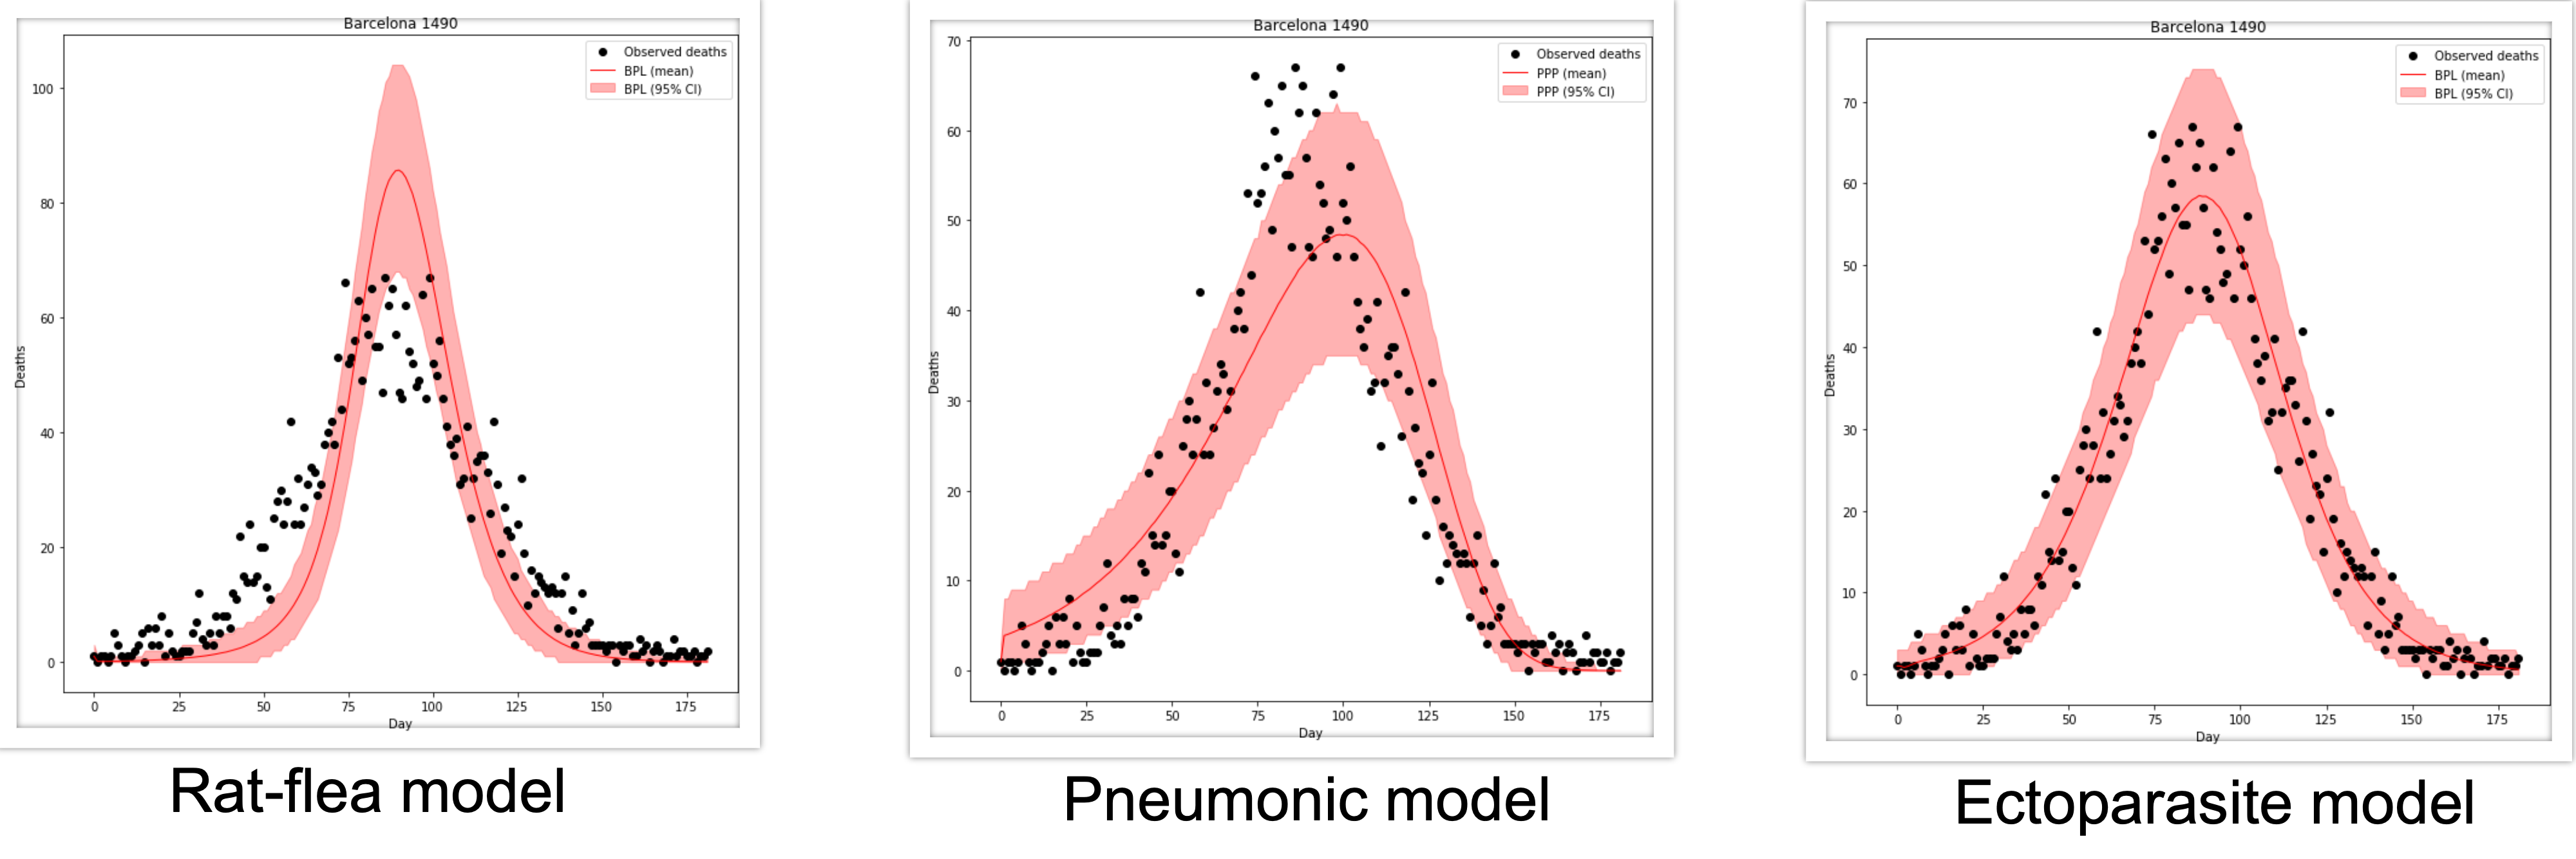
\includegraphics[width=\linewidth]{Figures/models1.png}
	\end{subfigure}\hspace{\fill}
	\caption{The black data points are recorded deaths pre day in the given data set. As is visible, the human-ecto model does get the closest to fitting the given data} 
\end{figure}

Here for example for above
\begin{figure}[h!]
	\begin{subfigure}{0.48\textwidth}
	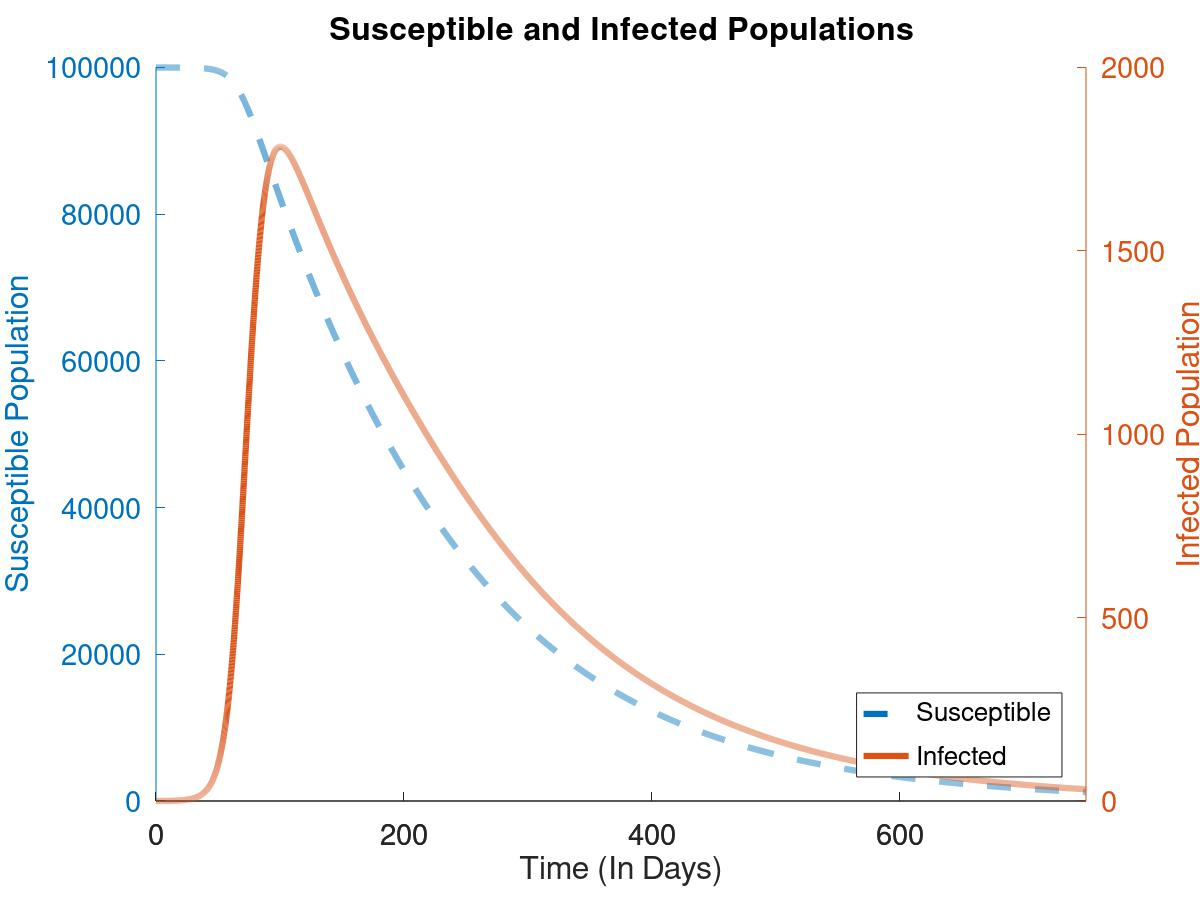
\includegraphics[width=\linewidth]{Figures/bubonic750.jpg}
	\end{subfigure}\hspace{\fill}
	\begin{subfigure}{0.48\textwidth}
	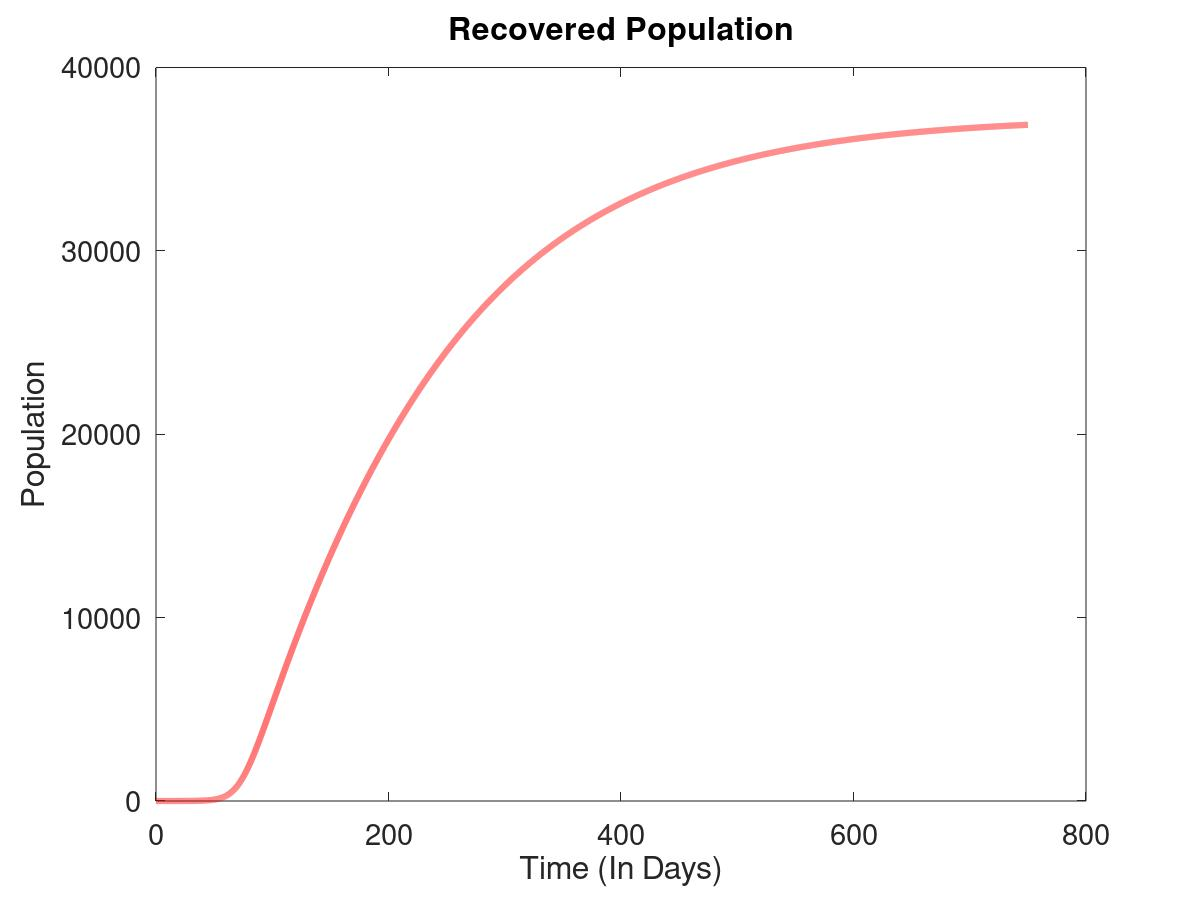
\includegraphics[width=\linewidth]{Figures/bubonicr.jpg}
	\end{subfigure}
	\begin{subfigure}{0.48\textwidth}
	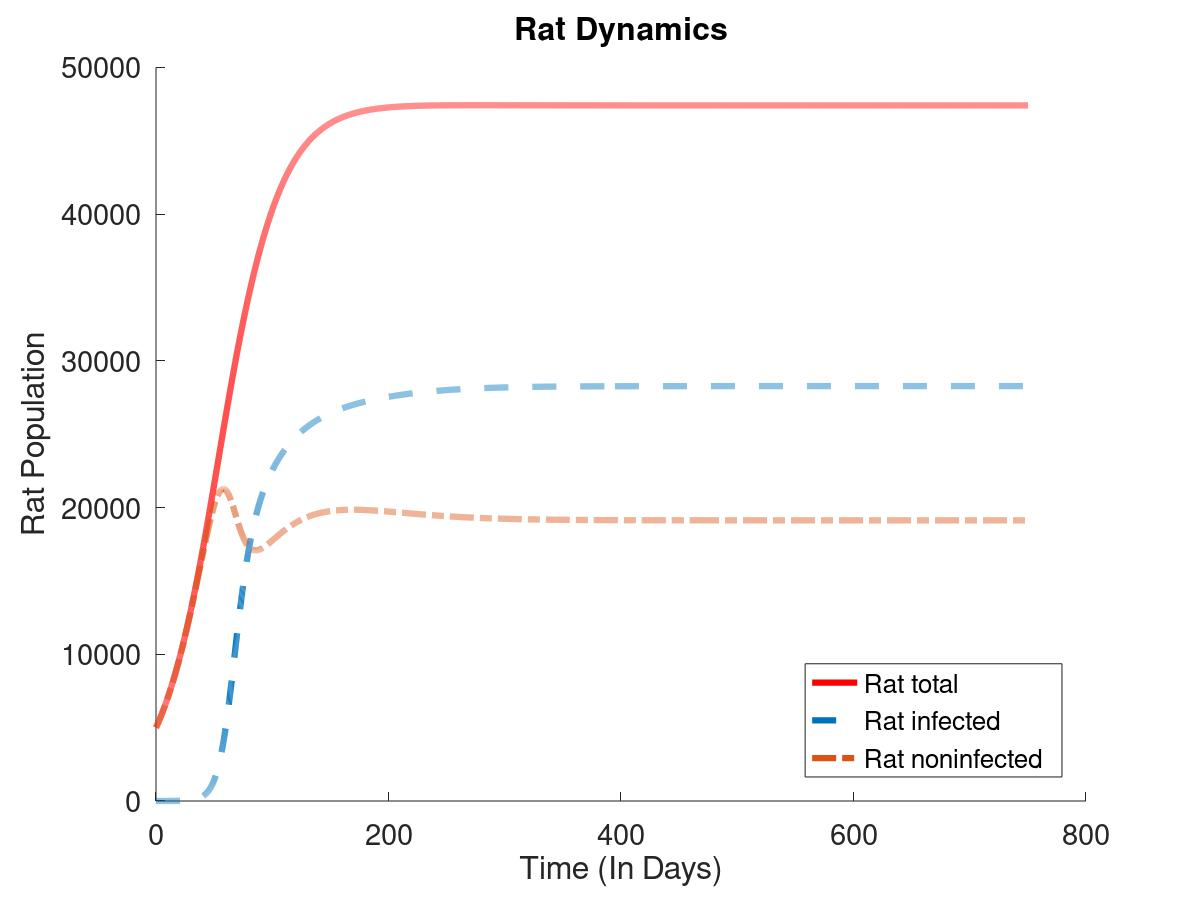
\includegraphics[width=\linewidth]{Figures/bubonicrat.jpg}
	\end{subfigure}\hspace{\fill}
	\begin{subfigure}{0.48\textwidth}
	\includegraphics[width=\linewidth]{Figures/Bubonicrf.jpg}
	\end{subfigure}
	\caption{Human, rat, and flea populations under the bubonic model. The parameters are $\alpha=0.25, \delta=1/300, \gamma=0.1, \lambda=0.2, \rho=1/40, \sigma=1.5*10^{-3}, \nu=1/6, \phi=1/6, r=1/10.$}
\end{figure}

\newpage

\section {Discussion}

Words... 




\pagebreak

\bibliography{References.bib}
\bibliographystyle{plain}

\end{document}